%% ======================================================================
%% PART 0 — PREAMBLE, TITLE, AUTHORS, ABSTRACT, INDEX TERMS
%% ======================================================================
\documentclass[conference]{IEEEtran}
\IEEEoverridecommandlockouts
\usepackage{cite}
\usepackage{amsmath,amssymb,amsfonts}
\usepackage{graphicx}
\usepackage{textcomp}
\usepackage{xcolor}
\usepackage{url}
\usepackage{array}
\usepackage{booktabs}
\usepackage{balance}
\usepackage{tikz}
\usetikzlibrary{arrows.meta,positioning,shapes.geometric,fit,calc}
\graphicspath{{figures/}{./}}

\tikzset{
  box/.style={draw, rounded corners=2pt, align=center, font=\scriptsize, inner sep=3pt, minimum height=0.55cm},
  store/.style={draw, cylinder, shape border rotate=90, aspect=0.18, align=center, font=\scriptsize, minimum height=0.85cm, minimum width=1.55cm},
  state/.style={draw, rounded corners=6pt, align=center, font=\scriptsize, minimum height=0.6cm, inner sep=3pt},
  arr/.style={-{Stealth[length=1.6mm]}, thin},
  lbl/.style={font=\tiny, align=center}
}

\begin{document}

\title{MedAccess: A Pharmacist-Supervised Platform for Medicine Availability, Price Comparison and Safe Brand Matching Using the Common Drug Codes for India%
\thanks{This work was carried out as the course software project for BCSE301L Software Engineering at Vellore Institute of Technology, Chennai, India.}}

\author{
\IEEEauthorblockN{Bhuvanesh Jatla}
\IEEEauthorblockA{\textit{Reg. No. 24BYB1113} \\
\textit{VIT Chennai}\\
Chennai, India}
\and
\IEEEauthorblockN{Akshit Sitaram}
\IEEEauthorblockA{\textit{Reg. No. 24BYB1111} \\
\textit{VIT Chennai}\\
Chennai, India}
\and
\IEEEauthorblockN{Shailesh P}
\IEEEauthorblockA{\textit{Reg. No. 24BYB1108} \\
\textit{VIT Chennai}\\
Chennai, India}
\and
\IEEEauthorblockN{Rishabh Sharma}
\IEEEauthorblockA{\textit{Reg. No. 23BRS1369} \\
\textit{VIT Chennai}\\
Chennai, India}
}

\maketitle

\begin{abstract}
Patients in India frequently cannot tell which nearby pharmacy stocks a prescribed medicine, what it costs there, or whether a cheaper brand with the same composition exists. Consumer applications that answer these questions tend to present lower-priced alternatives as interchangeable without professional oversight. This paper presents MedAccess, a role-based web platform that combines the national Common Drug Codes for India (CDCI) catalogue of 93{,}911 brands with pharmacy-reported availability and indicative prices, and that identifies \emph{potential} brand matches sharing an identical CDCI generic identifier. A match is treated as informational only until a pharmacist explicitly verifies or rejects it through an audited state machine. Controlled and narcotic substances are excluded at index-construction time by a reviewable, whole-word restricted-substance list, so that no role or route can return them. Every stock, price, verification and administrative action is attributed, time-stamped and recorded in an audit log, and stale availability data is flagged rather than presented as current. The prototype is implemented in Node.js with no third-party runtime dependencies, an in-memory search index and a modular route architecture. Evaluation with 95 automated tests, including real-browser and accessibility audits, shows median search latency of 33--77\,ms over 90{,}939 indexed brands, complete exclusion of 2{,}972 restricted brands (3.2\,\%), and full or partial satisfaction of all 39 functional requirements of the system specification.
\end{abstract}

\begin{IEEEkeywords}
medicine availability, price transparency, drug terminology, pharmacist verification, role-based access control, health information systems, audit logging
\end{IEEEkeywords}

%% ======================================================================
%% PART 1 — INTRODUCTION
%% ======================================================================
\section{Introduction}
Access to essential medicines depends not only on whether a medicine exists in the market but on whether a patient can find it at an affordable price in a nearby pharmacy. Cross-national surveys have repeatedly reported low public-sector availability and high, widely varying private-sector prices for essential medicines in low- and middle-income countries \cite{cameron2009,who2008}. In India, the same molecule at the same strength is typically marketed under many brand names by different manufacturers, with substantial price differences between brands; the Government's Jan Aushadhi programme was created precisely to make equivalent generic medicines available at lower cost \cite{pmbjp}.

Two practical information gaps follow from this situation. First, a patient or caregiver rarely knows which pharmacy currently stocks a medicine and at what price. Second, even when a lower-priced brand with the same composition exists, the patient has no safe way to establish that it is a suitable substitute. Ingredient name alone is insufficient: strength, dosage form, release mechanism and pack size all matter, and substitution decisions are a professional responsibility. Consumer tools that list ``cheaper alternatives'' automatically risk presenting a price comparison as a clinical equivalence claim.

This paper presents \emph{MedAccess}, developed as our software project for the course BCSE301L Software Engineering at VIT Chennai: a prototype platform designed around a different principle: the system may \emph{identify} candidate matches, but only a pharmacist may \emph{verify} them. The main contributions are:
\begin{enumerate}
\item A catalogue-grounded matching method that proposes potential brand matches only when two brands share an identical CDCI generic identifier (same ingredients, strength and dosage form), and that exposes the remaining differences (manufacturer, pack size, price per unit) instead of hiding them.
\item An explicit pharmacist-verification workflow, modelled as a state machine with attributed, time-stamped and audited transitions, in which no comparison can become ``verified'' without a human decision.
\item A fail-closed exclusion mechanism for controlled and narcotic substances, applied once when the search index is built, so that excluded brands are unreachable through every role and every API route.
\item A provenance-aware availability and price model that merges read-only seed data with attributed staff updates and flags stale records, together with a modular, dependency-free implementation evaluated with 95 automated tests.
\end{enumerate}

The remainder of the paper is organised as follows. Section~\ref{sec:related} reviews related work. Section~\ref{sec:req} summarises requirements and design constraints. Section~\ref{sec:arch} describes the architecture, and Section~\ref{sec:mech} the core mechanisms. Section~\ref{sec:impl} covers implementation, Section~\ref{sec:eval} the evaluation, and Section~\ref{sec:disc} limitations. Section~\ref{sec:concl} concludes.

%% ======================================================================
%% PART 2 — RELATED WORK
%% ======================================================================
\section{Related Work}\label{sec:related}

\subsection{Medicine Prices and Availability}
The WHO/Health Action International methodology \cite{who2008} standardised the measurement of medicine prices, availability and affordability through facility surveys, and its application across 36 countries documented poor availability and large price mark-ups \cite{cameron2009}. These studies establish the problem but are periodic surveys; they do not provide patients with current, pharmacy-level information. MedAccess addresses the latter while keeping the provenance and age of each data point visible.

\subsection{Drug Terminology and Catalogues}
Reliable comparison requires a controlled vocabulary in which a brand is linked to a generic concept with a defined strength and dosage form. The Common Drug Codes for India (CDCI), maintained by the National Resource Centre for EHR Standards (NRCeS), provides national identifiers for generics, products, brands and suppliers \cite{cdci}. MedAccess uses CDCI as its authoritative reference and deliberately limits automatic matching to the generic identifier that CDCI itself assigns, rather than to free-text name similarity.

\subsection{Generic Medicine Programmes and Consumer Applications}
Government initiatives such as Pradhan Mantri Bhartiya Janaushadhi Pariyojana promote quality generic medicines at reduced prices \cite{pmbjp}. Commercial e-pharmacy and price-comparison applications commonly list lower-priced substitutes, but they couple discovery with sales and seldom record who, if anyone, confirmed that a substitute is appropriate. MedAccess intentionally excludes sales, payment and delivery, and separates informational matching from professional verification.

\subsection{Access Control and Accountability in Health Systems}
Role-based access control (RBAC) \cite{sandhu1996,ferraiolo2001} is the established model for health information systems in which permissions follow professional roles. Accountability additionally requires that changes be attributable and auditable, and common web-application risks such as broken access control and injection remain the leading vulnerability classes \cite{owasp2021}. MedAccess applies route-level RBAC with per-request account-status checks, parameterised SQL and a before/after audit trail. Synthetic data is used throughout, following the practice of using realistic synthetic records to develop health software without exposing real patients \cite{synthea}.

%% ======================================================================
%% PART 3 — REQUIREMENTS AND DESIGN CONSTRAINTS
%% ======================================================================
\section{Requirements and Design Constraints}\label{sec:req}

\subsection{Stakeholders and Elicitation}
Structured questionnaires were prepared for seven stakeholder groups (patients, caregivers, doctors, pharmacists, pharmacy staff, pharmacies and administrators). For this academic prototype the responses were simulated from the perspective of each group, and the resulting needs were consolidated into a Software Requirements Specification (SRS) in line with the guidance of ISO/IEC/IEEE 29148 \cite{iso29148}. The SRS defines 39 functional requirements (FR), 18 non-functional requirements (NFR) and 10 business rules (BR), and was accompanied by UML use-case, activity, sequence, state and entity--relationship models.

\subsection{Functional Scope}
The functional requirements group into nine areas: authentication and roles; medicine search and details; pharmacy availability; indicative prices and comparison; potential matching and pharmacist verification; stock and price updates; incorrect-information reports; refill reminders; and administration (users, catalogue, reports and audit). Table~\ref{tab:roles} summarises the capabilities granted to each of the six roles.

\begin{table}[!t]
\caption{Role--Capability Matrix}
\label{tab:roles}
\centering
\scriptsize
\setlength{\tabcolsep}{3pt}
\begin{tabular}{@{}lcccccc@{}}
\toprule
Capability & Pat. & Care. & Phar. & Staff & Admin & Doc. \\
\midrule
Search catalogue / details        & \checkmark & \checkmark & \checkmark & \checkmark & \checkmark & \checkmark \\
View availability and prices      & \checkmark & \checkmark & \checkmark & \checkmark & \checkmark & -- \\
View potential matches            & \checkmark & \checkmark & \checkmark & -- & -- & \checkmark \\
Request pharmacist verification   & \checkmark & \checkmark & \checkmark & -- & -- & -- \\
Verify / reject a comparison      & -- & -- & \checkmark & -- & -- & -- \\
Update stock and price            & -- & -- & \checkmark & \checkmark & -- & -- \\
Submit incorrect-info report      & \checkmark & \checkmark & \checkmark & \checkmark & -- & -- \\
Review and resolve reports        & -- & -- & \checkmark & \checkmark & \checkmark & -- \\
Refill reminders                  & \checkmark & \checkmark & -- & -- & -- & -- \\
Users, catalogue, reports, audit  & -- & -- & -- & -- & \checkmark & -- \\
\bottomrule
\end{tabular}
\end{table}

\subsection{Safety and Business Rules}
Four business rules shape the design more than any other requirement. A potential match is informational only (BR-01); only a pharmacist may verify it (BR-02); a lower price does not imply suitability (BR-03); and controlled, narcotic and psychotropic medicines are outside the scope of the system (BR-07), consistent with their special regulatory status under the Narcotic Drugs and Psychotropic Substances Act \cite{ndps}. The system also performs no diagnosis or prescribing (BR-06) and no sales, payment or delivery (BR-08).

\subsection{Non-Functional Requirements}
Key NFRs are server-side authorisation (NFR-01--04), minimal personal data and synthetic demonstration data (NFR-06, NFR-07), mobile-friendly and accessible presentation (NFR-09, NFR-11), source and time on every availability and price value (NFR-13), never presenting stale data as current (NFR-14), traceability of changes (NFR-16) and a modular structure (NFR-18). Accessibility was assessed against WCAG~2.1 success criteria \cite{wcag21}.

%% ======================================================================
%% PART 4 — SYSTEM ARCHITECTURE
%% ======================================================================
\section{System Architecture}\label{sec:arch}

\subsection{Overview}
MedAccess follows a three-tier architecture (Fig.~\ref{fig:arch}). A single-page client built from plain ES modules communicates with a JSON API over HTTP. The server is organised as a composition root that builds a shared \emph{kernel} (database helpers, audit writer, route registry, role constants and reference stores) and registers ten component modules, one per functional area, each declaring its routes as \texttt{route(method, path, roles, handler)}. Data is held in four stores: an application database, the read-only CDCI catalogue, a read-only synthetic inventory, and an in-memory search index derived from the catalogue.

\begin{figure*}[!t]
\centering
\resizebox{\textwidth}{!}{%
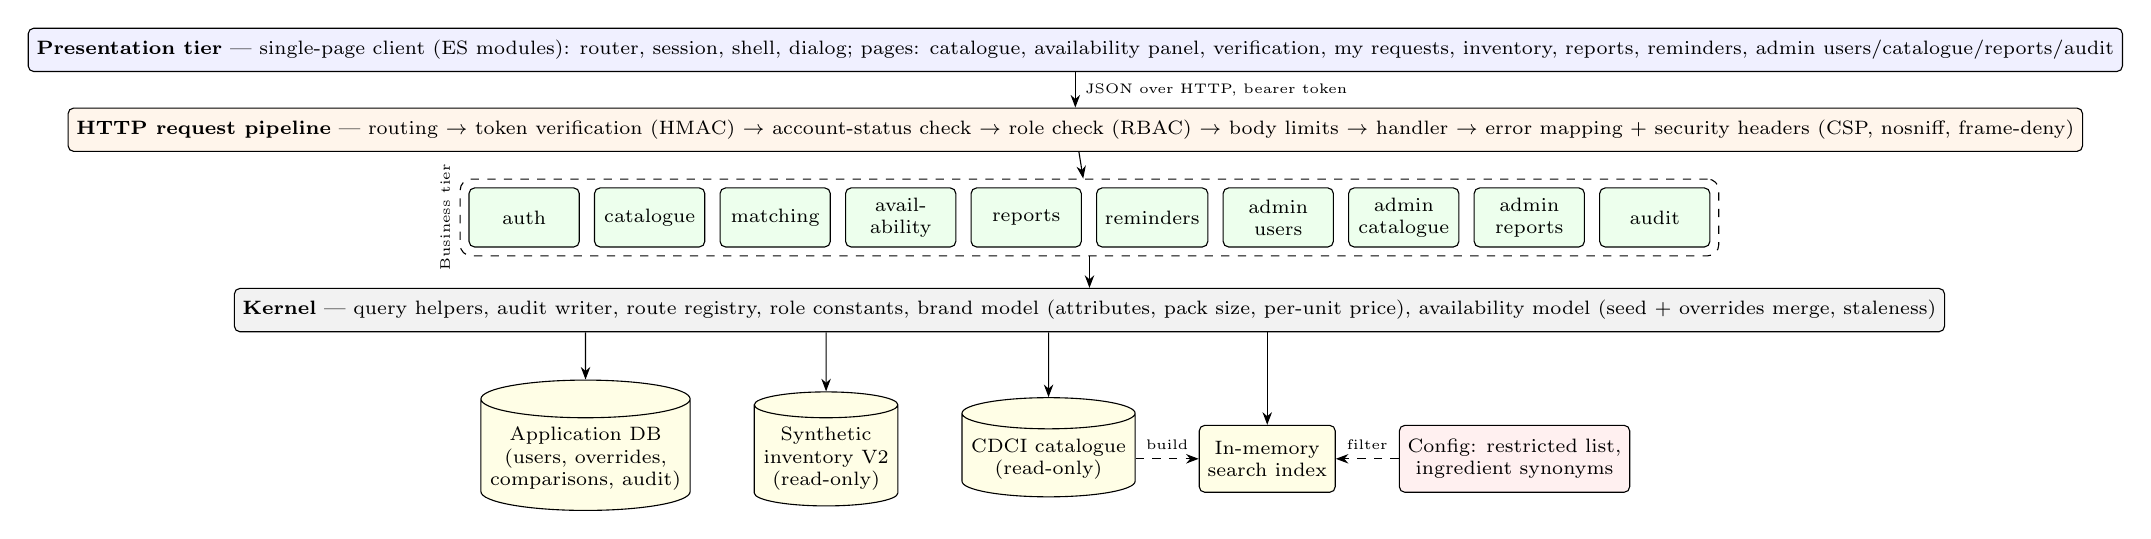
\begin{tikzpicture}[node distance=0.35cm and 0.3cm]
% client tier
\node[box, fill=blue!6, minimum width=16.6cm] (client) {\textbf{Presentation tier} --- single-page client (ES modules): router, session, shell, dialog; pages: catalogue, availability panel, verification, my requests, inventory, reports, reminders, admin users/catalogue/reports/audit};
% pipeline
\node[box, fill=orange!8, minimum width=16.6cm, below=0.45cm of client] (pipe) {\textbf{HTTP request pipeline} --- routing $\rightarrow$ token verification (HMAC) $\rightarrow$ account-status check $\rightarrow$ role check (RBAC) $\rightarrow$ body limits $\rightarrow$ handler $\rightarrow$ error mapping + security headers (CSP, nosniff, frame-deny)};
% components
\node[box, fill=green!7, below=0.45cm of pipe, xshift=-7.0cm, minimum width=1.4cm, minimum height=0.75cm] (c1) {auth};
\node[box, fill=green!7, right=0.18cm of c1, minimum width=1.4cm, minimum height=0.75cm] (c2) {catalogue};
\node[box, fill=green!7, right=0.18cm of c2, minimum width=1.4cm, minimum height=0.75cm] (c3) {matching};
\node[box, fill=green!7, right=0.18cm of c3, minimum width=1.4cm, minimum height=0.75cm] (c4) {avail-\\ability};
\node[box, fill=green!7, right=0.18cm of c4, minimum width=1.4cm, minimum height=0.75cm] (c5) {reports};
\node[box, fill=green!7, right=0.18cm of c5, minimum width=1.4cm, minimum height=0.75cm] (c6) {reminders};
\node[box, fill=green!7, right=0.18cm of c6, minimum width=1.4cm, minimum height=0.75cm] (c7) {admin\\users};
\node[box, fill=green!7, right=0.18cm of c7, minimum width=1.4cm, minimum height=0.75cm] (c8) {admin\\catalogue};
\node[box, fill=green!7, right=0.18cm of c8, minimum width=1.4cm, minimum height=0.75cm] (c9) {admin\\reports};
\node[box, fill=green!7, right=0.18cm of c9, minimum width=1.4cm, minimum height=0.75cm] (c10) {audit};
\node[draw, dashed, rounded corners, fit=(c1)(c10), inner sep=3pt] (comp) {};
\node[font=\tiny, rotate=90, anchor=south] at (comp.west) {Business tier};
% kernel
\node[box, fill=gray!10, minimum width=16.6cm, below=0.4cm of comp] (kernel) {\textbf{Kernel} --- query helpers, audit writer, route registry, role constants, brand model (attributes, pack size, per-unit price), availability model (seed + overrides merge, staleness)};
% stores
\node[store, fill=yellow!10, below=0.6cm of kernel, xshift=-6.4cm] (appdb) {Application DB\\(users, overrides,\\comparisons, audit)};
\node[store, fill=yellow!10, right=0.8cm of appdb] (inv) {Synthetic\\inventory V2\\(read-only)};
\node[store, fill=yellow!10, right=0.8cm of inv] (cdci) {CDCI catalogue\\(read-only)};
\node[box, fill=yellow!10, right=0.8cm of cdci, minimum height=0.85cm] (idx) {In-memory\\search index};
\node[box, fill=red!6, right=0.8cm of idx, minimum height=0.85cm] (cfg) {Config: restricted list,\\ingredient synonyms};
% arrows
\draw[arr] (client) -- node[lbl, right]{JSON over HTTP, bearer token} (pipe);
\draw[arr] (pipe) -- (comp);
\draw[arr] (comp) -- (kernel);
\draw[arr] (kernel.south -| appdb) -- (appdb);
\draw[arr] (kernel.south -| cdci) -- (cdci);
\draw[arr] (kernel.south -| inv) -- (inv);
\draw[arr] (kernel.south -| idx) -- (idx);
\draw[arr, dashed] (cdci.east) -- node[lbl, above]{build} (idx.west);
\draw[arr, dashed] (cfg.west) -- node[lbl, above]{filter} (idx.east);
\end{tikzpicture}%
}
\caption{Layered architecture of MedAccess. Each business component registers its own routes on the kernel; reference data is opened read-only and indexed once at start-up.}
\label{fig:arch}
\end{figure*}

\subsection{Request Pipeline and Security}
Every request passes through the same pipeline. Bearer tokens are HMAC-signed \cite{rfc2104} and valid for eight hours, and the account status is re-read from the database on every request so that deactivating an account takes effect immediately. Each route declares the roles allowed to call it, so authorisation is enforced on the server rather than by hiding user-interface elements. Passwords are hashed with scrypt \cite{percival2009}, login attempts are throttled after five failures, all SQL statements are parameterised, and responses carry Content-Security-Policy, \texttt{nosniff} and frame-deny headers, addressing the OWASP classes of broken access control and injection \cite{owasp2021}. Every login, denied access and data change is written to the audit log with actor, time, affected record and, for updates, the before and after values.

\subsection{Data Stores}
The application database (SQLite \cite{sqlite}) holds users and roles, staff stock and price updates, catalogue overlay entries, comparison records and comments, reports, reminders and the audit log. The CDCI catalogue and the synthetic inventory are opened read-only; the application never writes to them. Staff updates are therefore stored as \emph{overrides} that are merged with the seed at read time (Section~\ref{sec:mech}-D), and administrator corrections to the catalogue are stored as an \emph{overlay} that can hide or annotate a brand, record its pack size, or add a brand that CDCI does not list.

\subsection{Client}
The client is a framework-free single-page application served as static ES modules, with one module per page and a hash router that enforces login and role access before rendering. Each data value is rendered with its origin and age, safety notices accompany every match list, and the layout reflows down to 320\,px in both light and dark themes.

%% ======================================================================
%% PART 5 — CORE MECHANISMS
%% ======================================================================
\section{Core Mechanisms}\label{sec:mech}

\subsection{Catalogue Indexing and Restricted-Substance Exclusion}
Fig.~\ref{fig:pipeline} shows how the catalogue becomes searchable. At start-up each CDCI brand row is joined with its generic and dosage-form master records and tested against the restricted list $L$, which contains 65 substances and a classification rule. Let $\mathrm{tok}(b)$ be the set of word tokens in the generic, product and brand names of brand $b$, and $\mathrm{cls}(b)$ its CDCI classification. The excluded set is
\begin{equation}
R=\{\,b \mid \exists s\in L:\ \mathrm{w}(s)\sqsubseteq \mathrm{tok}(b)\,\}\ \cup\ \{\,b \mid \mathrm{cls}(b)\in K\,\},
\label{eq:restricted}
\end{equation}
where $\mathrm{w}(s)\sqsubseteq \mathrm{tok}(b)$ means that the words of substance $s$ occur contiguously among the tokens of $b$, and $K$ is the set of restricted classifications. Brands in $R$ are never inserted into the index, so no route can return them. Matching is whole-word: \emph{morphine} excludes morphine products but not \emph{apomorphine}, a non-narcotic dopamine agonist. If the list is missing or malformed the server refuses to start (fail-closed). Administrators can see how many brands each entry removes, which supports review of the list by a pharmacist.

\begin{figure}[!t]
\centering
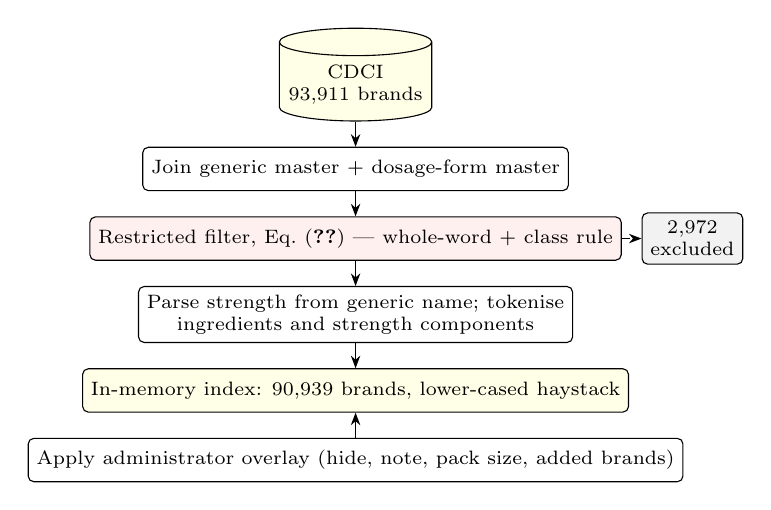
\begin{tikzpicture}[node distance=0.32cm]
\node[store, fill=yellow!10] (cdci) {CDCI\\93{,}911 brands};
\node[box, below=of cdci, minimum width=5.4cm] (join) {Join generic master + dosage-form master};
\node[box, fill=red!6, below=of join, minimum width=5.4cm] (filt) {Restricted filter, Eq.~(\ref{eq:restricted}) --- whole-word + class rule};
\node[box, below=of filt, minimum width=5.4cm] (parse) {Parse strength from generic name; tokenise\\ingredients and strength components};
\node[box, fill=yellow!10, below=of parse, minimum width=5.4cm] (idx) {In-memory index: 90{,}939 brands, lower-cased haystack};
\node[box, below=of idx, minimum width=5.4cm] (ov) {Apply administrator overlay (hide, note, pack size, added brands)};
\node[box, right=0.25cm of filt, fill=gray!10] (drop) {2{,}972\\excluded};
\draw[arr] (cdci) -- (join); \draw[arr] (join) -- (filt); \draw[arr] (filt) -- (parse);
\draw[arr] (parse) -- (idx); \draw[arr] (ov) -- (idx);
\draw[arr, dashed] (filt) -- (drop);
\end{tikzpicture}
\caption{Start-up pipeline that builds the searchable catalogue. Excluded brands never enter the index.}
\label{fig:pipeline}
\end{figure}

\subsection{Search, Attribute Parsing and Filters}
A substring scan with SQL \texttt{LIKE} over the joined catalogue view took about 0.67\,s per query on the test machine, so the searchable columns are copied once into an in-memory table with a lower-cased haystack and queried with \texttt{instr()}. Users may combine free text with separate active-ingredient, strength and dosage-form filters. Dosage form is taken from CDCI's structured form master; strength is parsed from the generic name and is labelled as unverified. A strength filter such as ``50'' matches only the numeric component of a strength token, so that it finds 50\,mg/5\,mL but not 500\,mg. A reviewable synonym list (e.g., paracetamol and acetaminophen) widens ingredient search without affecting matching.

\subsection{Potential Matching and Pharmacist Verification}
For a selected brand $b$ with CDCI generic identifier $g(b)$, the set of potential matches is
\begin{equation}
M(b)=\{\,b' \in C\setminus(R\cup H) \mid g(b')=g(b),\ b'\neq b\,\},
\label{eq:match}
\end{equation}
where $C$ is the catalogue and $H$ the set of brands hidden by an administrator. Because a CDCI generic identifier encodes ingredients, strength and dosage form together, members of $M(b)$ share all three by construction. For each match the system reports what still differs: brand, manufacturer and pack size (same, differs or unknown), together with the lowest demonstration price and, when the pack size begins with a unit count, an approximate price per unit.

A match carries no claim of equivalence until a user requests verification. The request creates a comparison record whose life cycle follows the state machine in Fig.~\ref{fig:states}, modelled after the statechart notation \cite{harel1987}. Only a pharmacist can start a review, verify or reject, and each terminal transition records the reviewer, the time and an optional comment. A rejected pair may be requested again, creating a new record and preserving the history. The requester follows progress on a \emph{My verification requests} page that shows the current status and the pharmacist's latest comment.

\begin{figure}[!t]
\centering
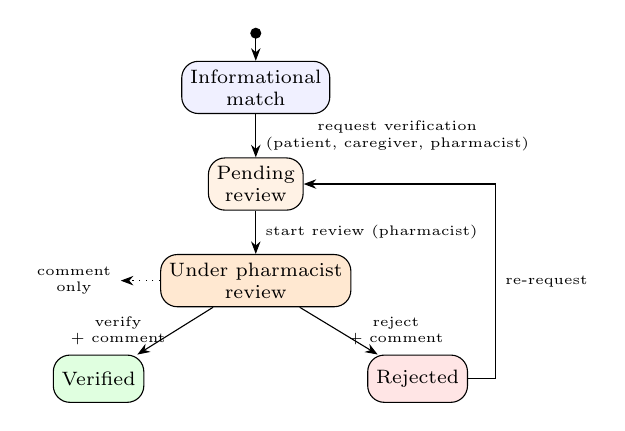
\begin{tikzpicture}[node distance=0.55cm and 0.4cm]
\node[state, fill=blue!6] (info) {Informational\\match};
\node[state, fill=orange!10, below=of info] (pend) {Pending\\review};
\node[state, fill=orange!18, below=of pend] (under) {Under pharmacist\\review};
\node[state, fill=green!12, below left=0.6cm and 0.2cm of under] (ver) {Verified};
\node[state, fill=red!10, below right=0.6cm and 0.2cm of under] (rej) {Rejected};
\fill ($(info.north)+(0,0.35)$) circle (2pt) coordinate (start);
\draw[arr] (start) -- (info);
\draw[arr] (info) -- node[lbl, right]{request verification\\(patient, caregiver, pharmacist)} (pend);
\draw[arr] (pend) -- node[lbl, right]{start review (pharmacist)} (under);
\draw[arr] (under) -- node[lbl, left]{verify\\+ comment} (ver);
\draw[arr] (under) -- node[lbl, right]{reject\\+ comment} (rej);
\draw[arr] (rej.east) -- ++(0.35,0) |- node[lbl, pos=0.25, right]{re-request} (pend.east);
\draw[arr, dotted] (under.west) -- ++(-0.5,0) node[lbl, left]{comment\\only} ;
\end{tikzpicture}
\caption{State machine of a brand comparison. Every transition is role-checked and audited; no transition to \emph{Verified} exists without pharmacist action.}
\label{fig:states}
\end{figure}

\subsection{Availability, Prices and Freshness}
Availability and price for a brand at a pharmacy are obtained by merging the read-only seed row with the newest staff override for that pair; the override wins and carries the updater's name, the time and the source label. Prices are stored as integer paise to avoid rounding errors and returned in rupees. A record $r$ with update time $t_r$ is flagged stale when
\begin{equation}
\mathrm{stale}(r) = \big[\, t_{\mathrm{now}} - t_r > \tau \,\big], \qquad \tau = 168\ \mathrm{h},
\label{eq:stale}
\end{equation}
and is then shown with a ``Possibly out of date'' badge instead of being presented as current (NFR-14). Because the synthetic seed has fixed timestamps, every seed row would eventually be stale. The demonstration therefore shifts each seed time by $\Delta = T_0 - \max_r t_r$, where $T_0$ is the server start time, which keeps the relative spread of the data while anchoring the newest row to the present. The shift is disclosed in the source label and in the API and can be disabled.

\subsection{Reports, Reminders and Audit}
Any patient, caregiver, pharmacist or staff member can report an incorrect price or availability for a specific brand and pharmacy. Reports move through \emph{Submitted}, \emph{Under Review}, \emph{Investigating} and then \emph{Resolved} or \emph{Rejected}, and resolution requires a note. Patients and caregivers can create one-time or recurring (daily, weekly, monthly) refill reminders, modify their time or recurrence, mark them done (which reschedules recurring reminders past the current time) or cancel them. All of these actions, like every administrative change, are written to the audit log.

%% ======================================================================
%% PART 6 — IMPLEMENTATION
%% ======================================================================
\section{Implementation}\label{sec:impl}

\subsection{Technology Stack}
The server runs on Node.js~22 \cite{nodejs} using only built-in modules: \texttt{node:http} for the server, \texttt{node:sqlite} for storage and \texttt{node:crypto} for hashing and token signing. The client uses no framework or build step. Avoiding third-party runtime dependencies removes supply-chain exposure and makes the prototype runnable with a single command. The code base comprises about 2{,}450 lines of server and client JavaScript and about 2{,}100 lines of tests.

\subsection{Modularity}
Following the information-hiding principle \cite{parnas1972}, the server is split into a 29-line composition root, a kernel, a request pipeline and ten component modules of 17--150 lines each that mirror the architecture diagram. A pinned route table (40 routes) guards against accidental changes: a test fails if any route is added, removed, reordered or re-protected without updating the snapshot, and a scripted scenario must exercise every route without a server error.

\subsection{Data}
The catalogue is the CDCI release used in the project (93{,}911 brands, 4{,}460 generics after exclusion). Pharmacy data is entirely synthetic: 20 fictional pharmacies in six Tamil Nadu cities with 875 inventory rows covering 120 brands. Every screen that shows this data carries a ``DEMO DATA --- NOT LIVE PHARMACY AVAILABILITY'' label. Six demonstration accounts, one per role, are seeded locally.

\subsection{User Interface}
Fig.~\ref{fig:ui-avail} shows the availability table for a losartan 50\,mg brand, with each status and price annotated with its age and source; the row updated by pharmacy staff names the staff member. Fig.~\ref{fig:ui-review} shows a comparison under pharmacist review, and Fig.~\ref{fig:ui-req} the requester's view of the same requests after the pharmacist's decision.

\begin{figure}[!t]
\centering
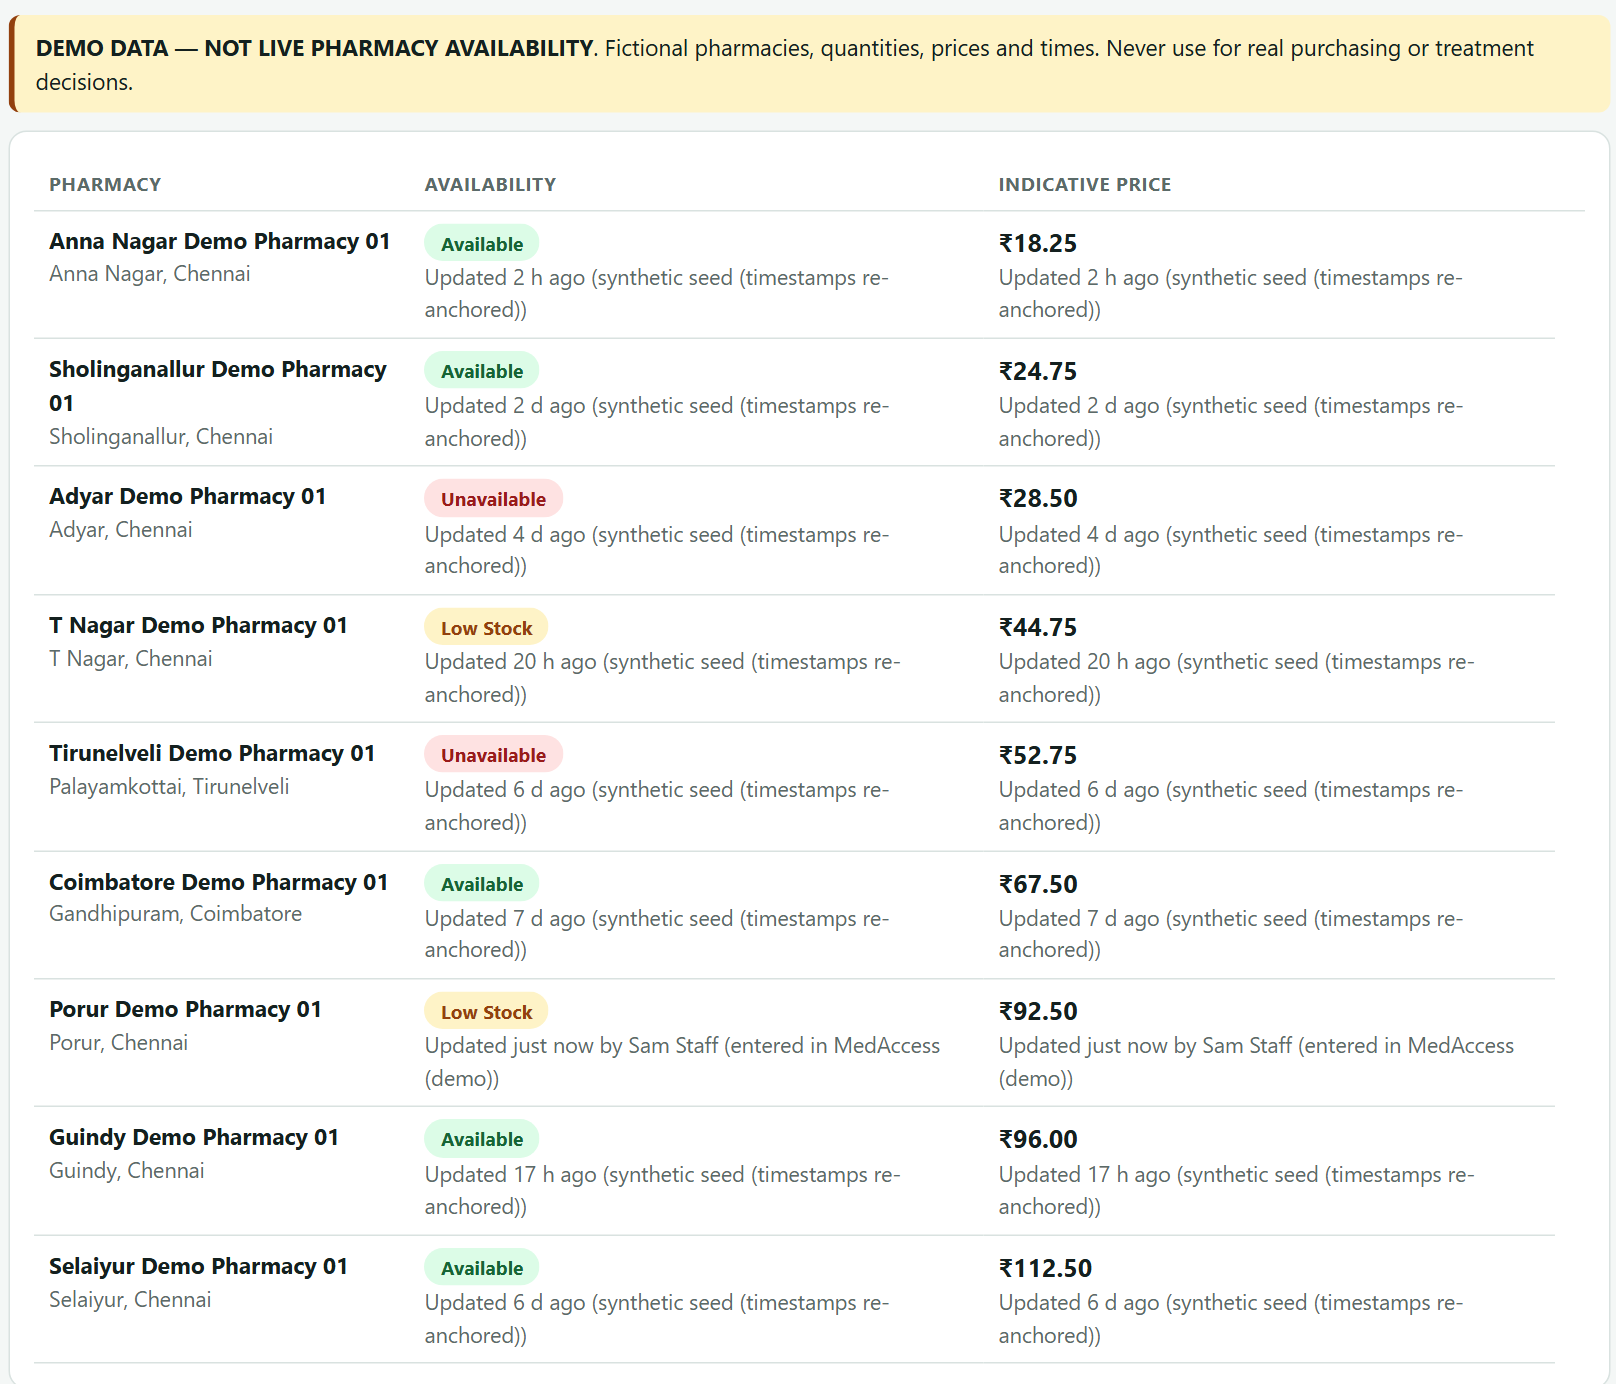
\includegraphics[width=\columnwidth]{fig_availability.png}
\caption{Availability and indicative prices for one brand across pharmacies, each with status, age and source. The ``entered in MedAccess'' row is a staff override that supersedes the seed value.}
\label{fig:ui-avail}
\end{figure}

\begin{figure}[!t]
\centering
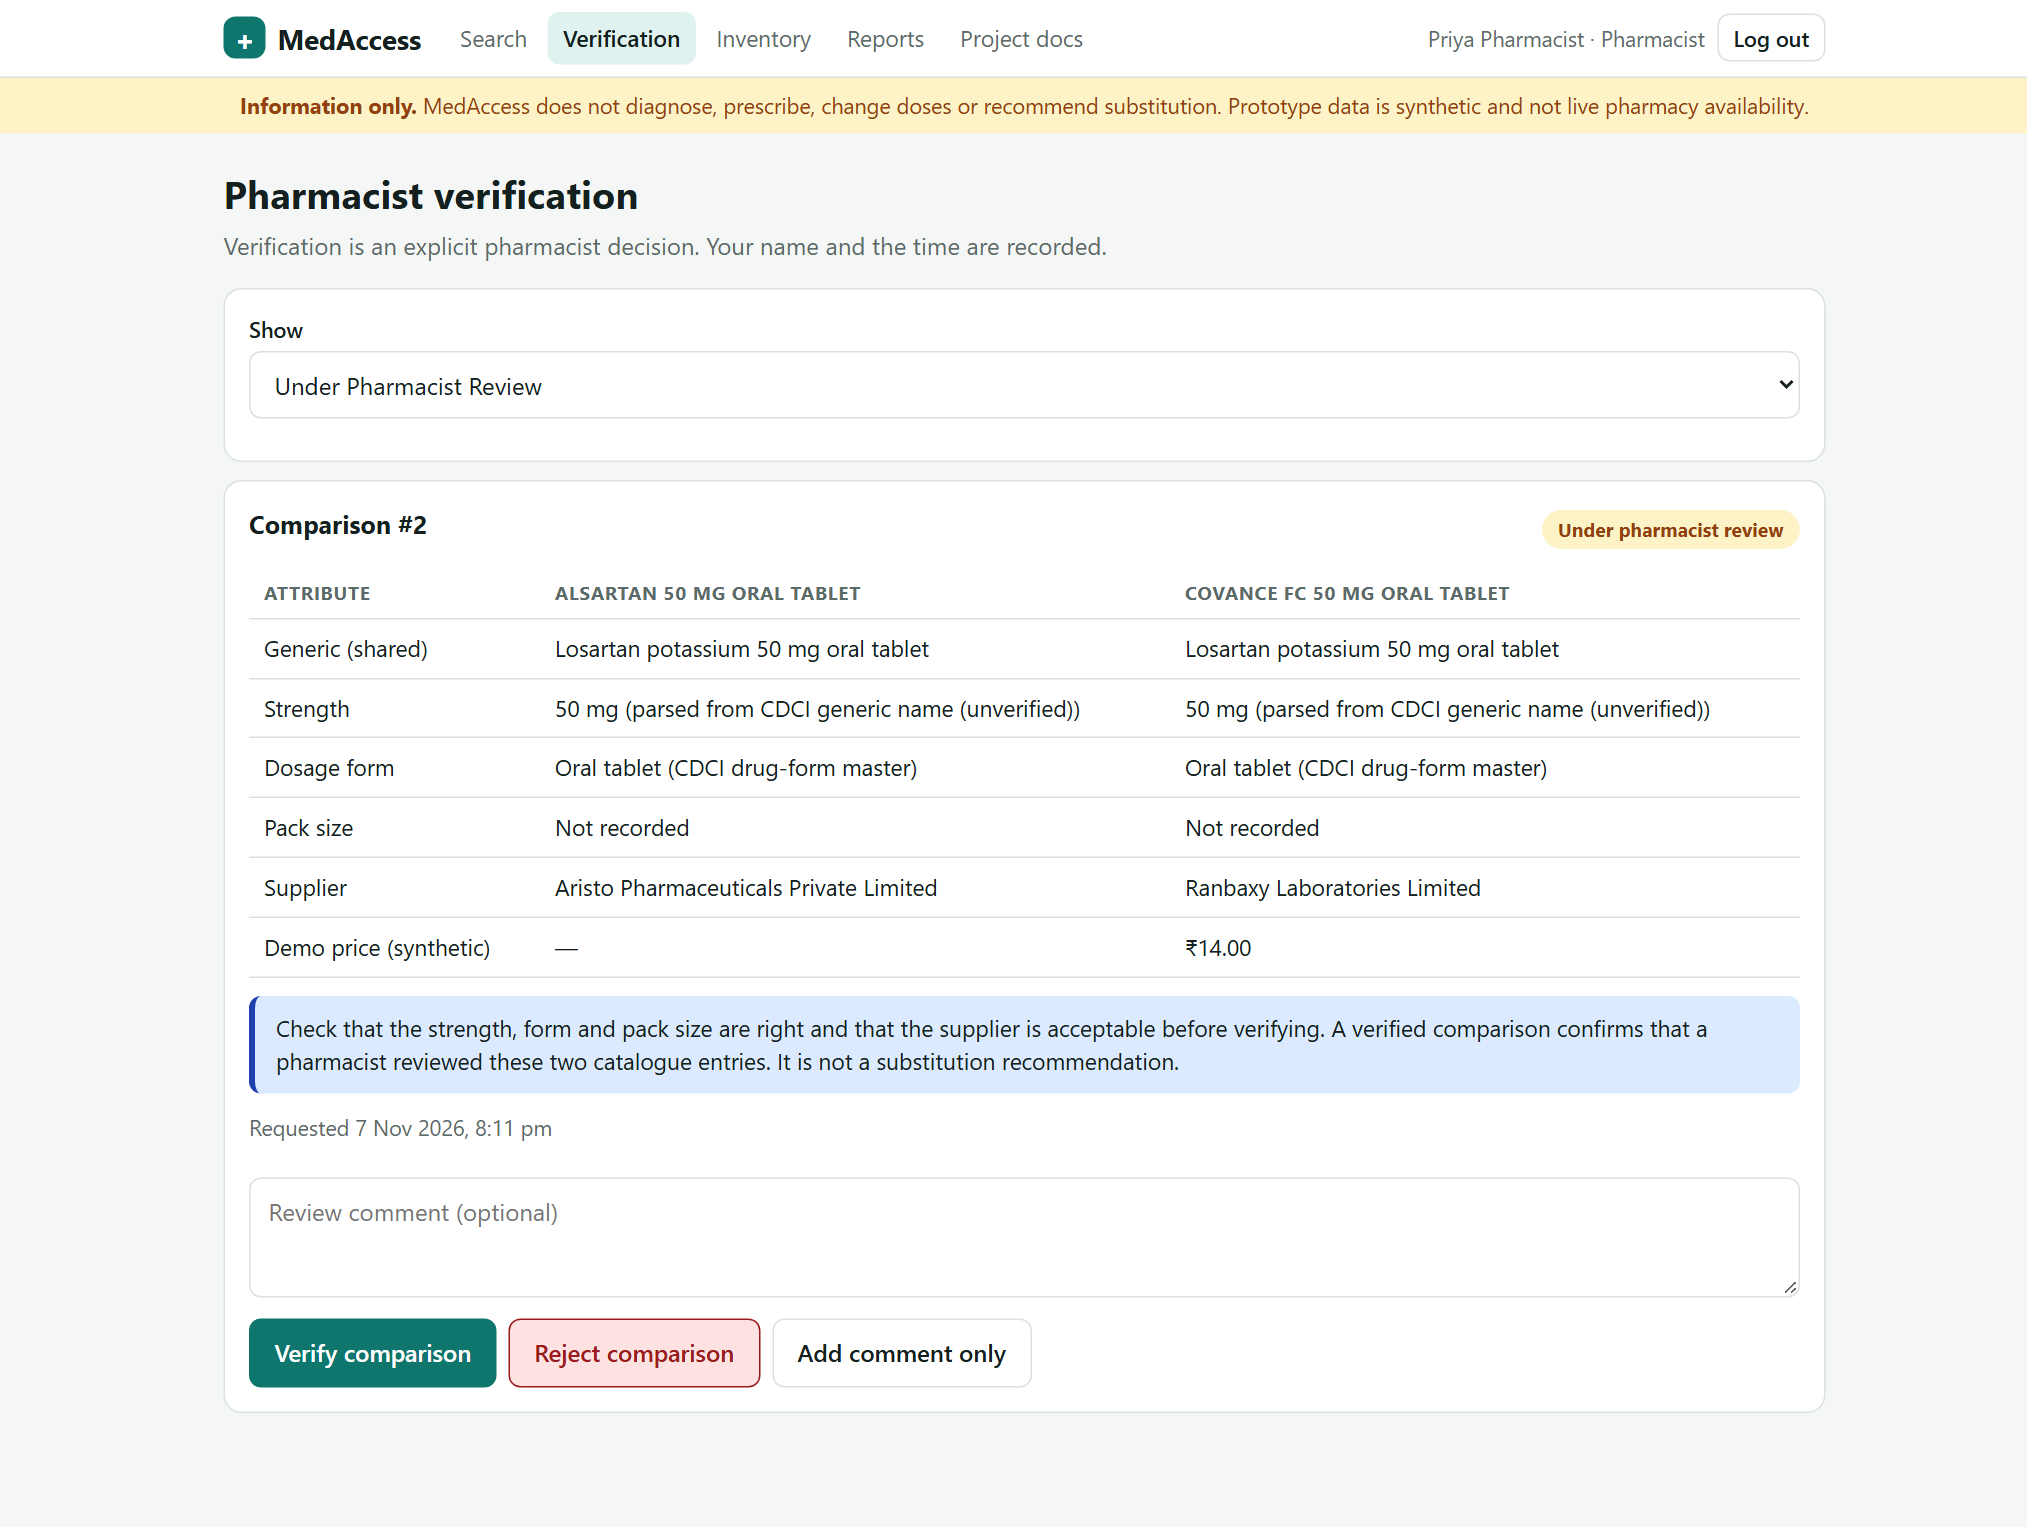
\includegraphics[width=\columnwidth]{fig_review.png}
\caption{Pharmacist review screen: attribute-by-attribute comparison of two brands with the safety notice, an optional comment, and the verify and reject actions.}
\label{fig:ui-review}
\end{figure}

\begin{figure}[!t]
\centering
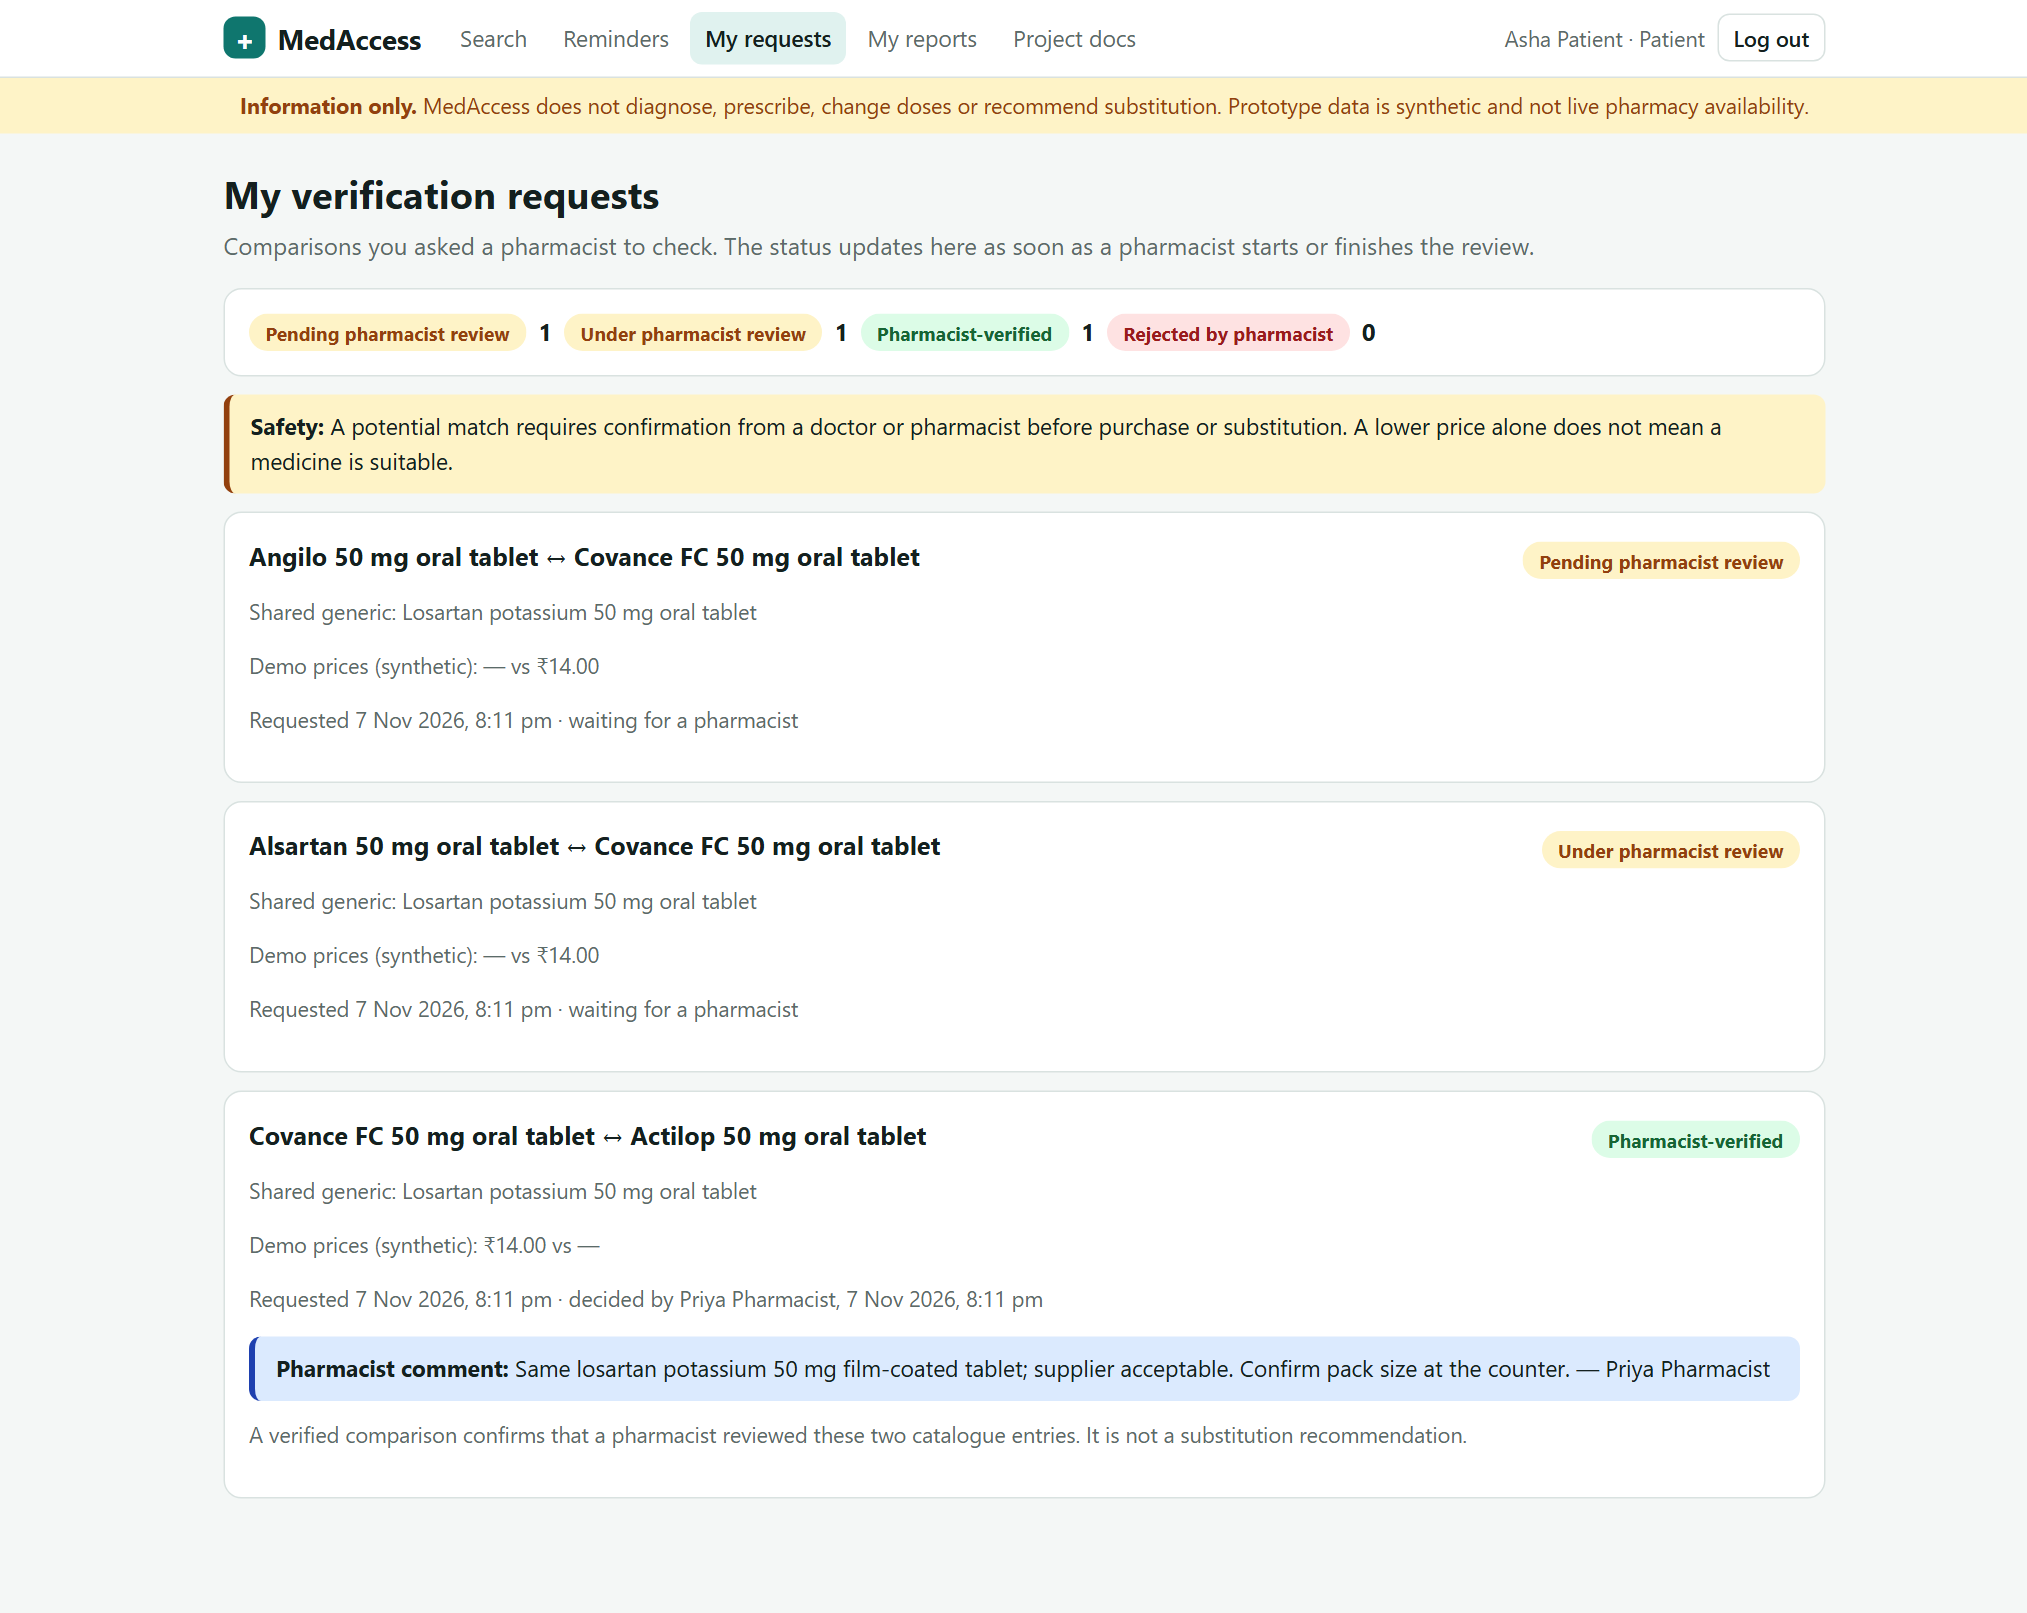
\includegraphics[width=\columnwidth]{fig_myrequests.png}
\caption{Requester's \emph{My verification requests} page showing pending, under-review and verified comparisons, with the reviewing pharmacist's name and comment.}
\label{fig:ui-req}
\end{figure}

%% ======================================================================
%% PART 7 — EVALUATION
%% ======================================================================
\section{Evaluation}\label{sec:eval}

\subsection{Test Methodology}
Correctness was evaluated with 95 automated tests run by the Node.js test runner (Table~\ref{tab:tests}). API tests start the real server on small fixture databases and assert status codes, role restrictions, state transitions and audit entries. Browser tests drive a headless Chromium-based browser through the DevTools protocol, sign in through the real login form and fail on any uncaught JavaScript error, console error or HTTP 5xx response. Accessibility tests audit each role's screens in light and dark themes for accessible names, headings, landmarks, table headers, keyboard reachability, target size and colour contrast, and exercise tab order, the skip link and the modal dialog. All 95 tests pass.

\begin{table}[!t]
\caption{Automated Test Suites}
\label{tab:tests}
\centering
\scriptsize
\begin{tabular}{@{}p{2.1cm}p{4.6cm}r@{}}
\toprule
Suite & Focus & Tests \\
\midrule
API            & RBAC, verification workflow, audit, validation & 6 \\
Reference      & CDCI catalogue, demo inventory, matching, re-anchoring & 8 \\
Parser         & Strength parsing from generic names & 11 \\
Restricted     & BR-07 exclusion across every route & 11 \\
Filters        & Ingredient, strength, form filters; synonyms & 11 \\
Overlay        & Hide, annotate, pack size, added brands & 7 \\
CSV import     & Pack-size bulk import with preview & 16 \\
Migration      & Upgrade of older databases & 2 \\
Routes         & Pinned route table; every route end to end & 3 \\
Browser        & Real-browser flows for all roles, mobile & 9 \\
Accessibility  & WCAG-oriented audit, light and dark, keyboard & 11 \\
\midrule
\multicolumn{2}{@{}l}{Total} & 95 \\
\bottomrule
\end{tabular}
\end{table}

\subsection{Performance}
Latency was measured on a consumer laptop (Windows~11, Node.js~22.18) with the full catalogue loaded, issuing 50 sequential authenticated requests per endpoint over the loopback interface. Table~\ref{tab:perf} reports the median and 95th percentile. Building the index at start-up took 4.8\,s. Free-text search over 90{,}939 brands completes in 51--77\,ms, compared with about 0.67\,s for a single \texttt{LIKE} scan over the source view, and the match and availability endpoints respond in under 4\,ms because they use indexed equality lookups.

\begin{table}[!t]
\caption{API Latency (50 Requests, Full Catalogue)}
\label{tab:perf}
\centering
\scriptsize
\begin{tabular}{@{}lrr@{}}
\toprule
Endpoint & p50 (ms) & p95 (ms) \\
\midrule
Search ``losartan''                         & 51.2 & 54.6 \\
Search ``paracetamol''                      & 76.8 & 78.5 \\
Filters: metformin, 500, tablet             & 33.3 & 34.6 \\
Potential matches (10 per page)             & 2.4  & 3.9 \\
Availability and prices for one brand       & 1.8  & 3.0 \\
\bottomrule
\end{tabular}
\end{table}

\subsection{Safety Validation}
The restricted list excluded 2{,}972 of 93{,}911 brands (3.2\,\%). Searches for tramadol, codeine and alprazolam returned no results, and the restricted-medicine suite verifies that excluded brands return \emph{not found} through every route: search, details, availability, matches, stock and price updates, reports, reminders, the overlay and the raw demonstration inventory. A search for ``morphine'' returned only three apomorphine products, confirming that whole-word matching avoids excluding unrelated substances. Workflow tests confirm that no comparison reaches \emph{Verified} without a pharmacist action, that non-pharmacist roles receive HTTP~403 on verification routes, and that each transition is audited with the reviewer and time.

\subsection{Requirements Coverage}
Each SRS requirement was traced to screens, routes and tests (Table~\ref{tab:cov}). All 39 functional requirements are met or partly met. The five partial ones depend on data or decisions outside the prototype: pack size (FR-07, FR-16) is supported but must be entered by administrators because CDCI does not record it; CDCI entries can be hidden or annotated but not edited (FR-08, FR-36); and the required administrative reports (FR-37) were not specified.

\begin{table}[!t]
\caption{SRS Coverage of the Implemented System}
\label{tab:cov}
\centering
\scriptsize
\begin{tabular}{@{}lrrrr@{}}
\toprule
Category & Total & Met & Partly & Not testable \\
\midrule
Functional (FR)       & 39 & 34 & 5 & 0 \\
Non-functional (NFR)  & 18 & 14 & 1 & 3 \\
Business rules (BR)   & 10 & 9  & 1 & 0 \\
\bottomrule
\end{tabular}
\end{table}

%% ======================================================================
%% PART 8 — DISCUSSION AND LIMITATIONS
%% ======================================================================
\section{Discussion and Limitations}\label{sec:disc}
The central design choice of MedAccess is to treat matching as a decision-support aid rather than a recommendation. Restricting automatic matching to an identical CDCI generic identifier sacrifices recall (for example, it will not pair two salts of the same base), but every proposed match shares ingredients, strength and dosage form by construction, and the remaining differences are shown explicitly. The pharmacist workflow converts each comparison into an accountable professional judgement.

Several limitations remain. Availability and prices are synthetic, and only 120 catalogue brands have demonstration inventory, and requirements were derived from simulated stakeholder responses, so the system has not been evaluated with live pharmacy data or real users; plain-language clarity and data-entry burden for pharmacy staff (NFR-10, NFR-12) therefore remain untested. The restricted-substance and synonym lists are drafts that require pharmacist review, and name-based matching can miss spellings the list does not contain. Strength is parsed from free-text names and labelled unverified. Reminders are shown in the application but are not delivered by SMS or e-mail. Finally, the prototype uses a single SQLite file and HTTP without TLS, and its audit log is not tamper-evident; production deployment would require TLS, a client--server database, persistent rate limiting and a hash-chained audit log.

%% ======================================================================
%% PART 9 — CONCLUSION, ACKNOWLEDGMENT, REFERENCES
%% ======================================================================
\section{Conclusion and Future Work}\label{sec:concl}
MedAccess shows that a national drug terminology can support useful availability, price and alternative-brand information for patients without allowing the software to make substitution decisions. Matching is constrained to identical CDCI generics, verification is reserved for pharmacists through an audited state machine, controlled substances are excluded before any query can reach them, and every data point carries its source and age. The prototype meets or partly meets all functional requirements of its specification, passes 95 automated tests, and answers catalogue searches in under 80\,ms.

Future work includes integration with real pharmacy inventory feeds, pharmacist review of the restricted and synonym lists, structured pack-size data from manufacturers, reminder delivery through SMS or e-mail, a ``request more information'' step in the verification workflow, and a field study with patients, caregivers and pharmacists to evaluate usability and the effect of verified comparisons on out-of-pocket spending.

\section*{Acknowledgment}
This work was completed as the software project for the course BCSE301L Software Engineering at Vellore Institute of Technology, Chennai. The authors thank the National Resource Centre for EHR Standards for making the Common Drug Codes for India available.

\balance
\begin{thebibliography}{00}
\bibitem{cameron2009} A. Cameron, M. Ewen, D. Ross-Degnan, D. Ball, and R. Laing, ``Medicine prices, availability, and affordability in 36 developing and middle-income countries: A secondary analysis,'' \textit{The Lancet}, vol. 373, no. 9659, pp. 240--249, Jan. 2009.
\bibitem{who2008} World Health Organization and Health Action International, \textit{Measuring Medicine Prices, Availability, Affordability and Price Components}, 2nd ed. Geneva, Switzerland: WHO, 2008.
\bibitem{pmbjp} Pharmaceuticals and Medical Devices Bureau of India, ``Pradhan Mantri Bhartiya Janaushadhi Pariyojana (PMBJP).'' [Online]. Available: \url{https://janaushadhi.gov.in}
\bibitem{cdci} National Resource Centre for EHR Standards (NRCeS), C-DAC Pune, ``Common Drug Codes for India (CDCI).'' [Online]. Available: \url{https://www.nrces.in}
\bibitem{sandhu1996} R. S. Sandhu, E. J. Coyne, H. L. Feinstein, and C. E. Youman, ``Role-based access control models,'' \textit{Computer}, vol. 29, no. 2, pp. 38--47, Feb. 1996.
\bibitem{ferraiolo2001} D. F. Ferraiolo, R. Sandhu, S. Gavrila, D. R. Kuhn, and R. Chandramouli, ``Proposed NIST standard for role-based access control,'' \textit{ACM Trans. Inf. Syst. Secur.}, vol. 4, no. 3, pp. 224--274, Aug. 2001.
\bibitem{owasp2021} OWASP Foundation, ``OWASP Top 10:2021.'' [Online]. Available: \url{https://owasp.org/Top10/}
\bibitem{synthea} J. Walonoski \textit{et al.}, ``Synthea: An approach, method, and software mechanism for generating synthetic patients and the synthetic electronic health care record,'' \textit{J. Amer. Med. Inform. Assoc.}, vol. 25, no. 3, pp. 230--238, Mar. 2018.
\bibitem{iso29148} \textit{Systems and Software Engineering---Life Cycle Processes---Requirements Engineering}, ISO/IEC/IEEE Standard 29148:2018, 2018.
\bibitem{ndps} Government of India, \textit{The Narcotic Drugs and Psychotropic Substances Act}, Act No. 61 of 1985.
\bibitem{wcag21} W3C, ``Web Content Accessibility Guidelines (WCAG) 2.1,'' W3C Recommendation, Jun. 2018. [Online]. Available: \url{https://www.w3.org/TR/WCAG21/}
\bibitem{rfc2104} H. Krawczyk, M. Bellare, and R. Canetti, ``HMAC: Keyed-hashing for message authentication,'' IETF RFC 2104, Feb. 1997.
\bibitem{percival2009} C. Percival, ``Stronger key derivation via sequential memory-hard functions,'' presented at BSDCan, Ottawa, Canada, May 2009.
\bibitem{sqlite} D. R. Hipp, ``SQLite.'' [Online]. Available: \url{https://www.sqlite.org}
\bibitem{harel1987} D. Harel, ``Statecharts: A visual formalism for complex systems,'' \textit{Sci. Comput. Program.}, vol. 8, no. 3, pp. 231--274, Jun. 1987.
\bibitem{nodejs} OpenJS Foundation, ``Node.js.'' [Online]. Available: \url{https://nodejs.org}
\bibitem{parnas1972} D. L. Parnas, ``On the criteria to be used in decomposing systems into modules,'' \textit{Commun. ACM}, vol. 15, no. 12, pp. 1053--1058, Dec. 1972.
\end{thebibliography}

\end{document}
